
\label{sec:ergebnisse}

\begin{figure}[!h]

	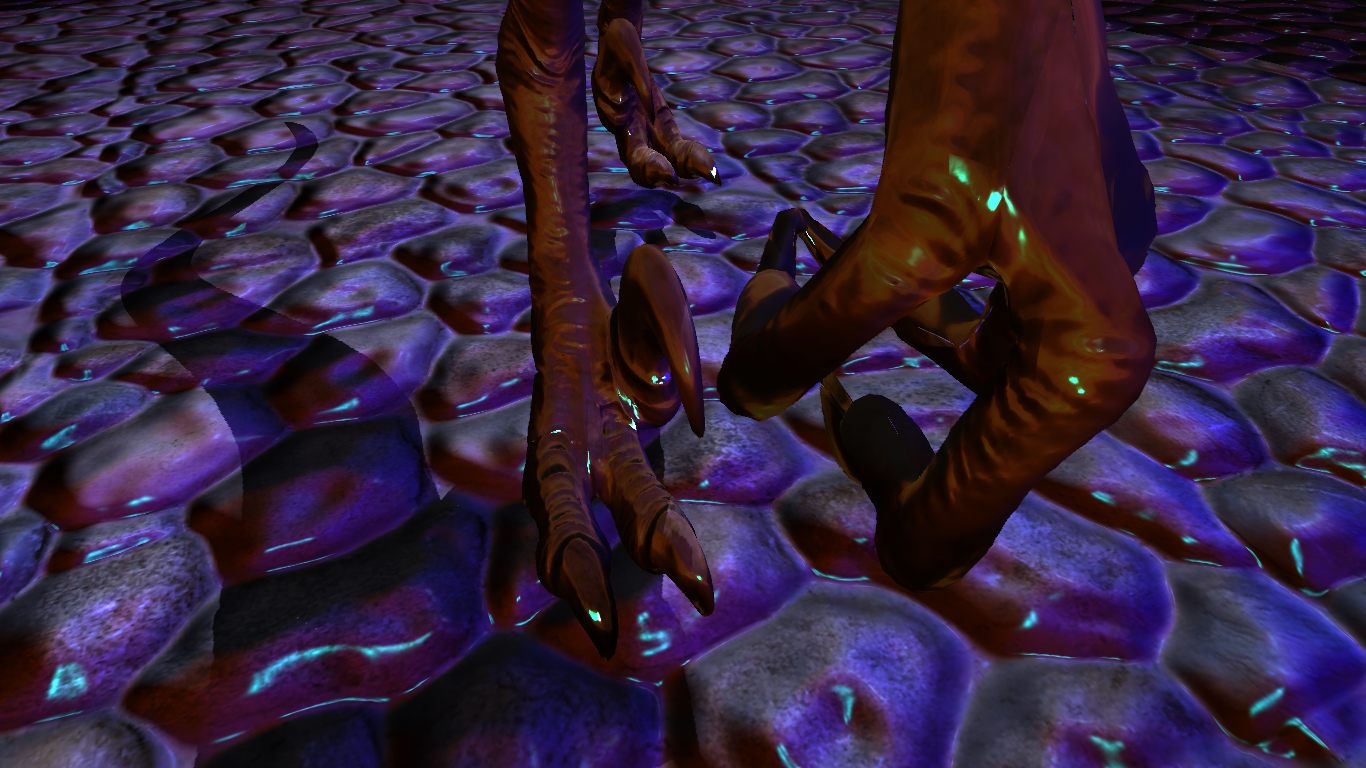
\includegraphics[width=1.2\textwidth]{Screenshot_raptorExtremities_allFX.png} 
	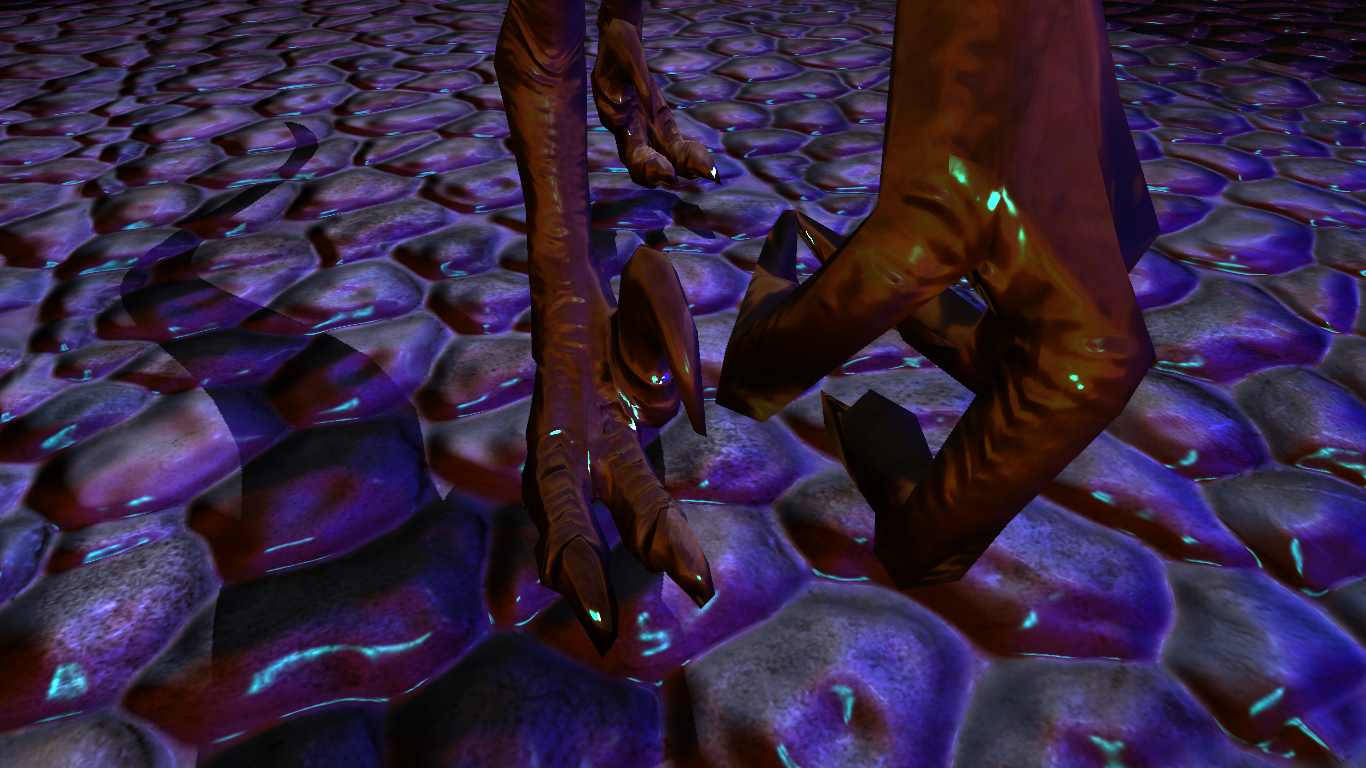
\includegraphics[width=1.2\textwidth]{Screenshot_raptorExtremities_allFX_withoutTess.png}

	\caption{Die Extremitäten des Raptor-modells; Oben: tesselliert, texturiert, normal mapped, environment mapped, 
	beleuchtet von fünf Lichtquellen , shadow mapped von einer Lichtquelle; Unten: wie oben, nur ohne Tessellation
	}
	\label{fig:raptorExtremitiesTessVSNonTess}
\end{figure}

Sämtliche Performance ist bisher rein GPU-limitiert, daher seien hier nur die
Graphikkarten der Systeme vorgestellt, mit denen \emph{Flewnit} getestet wurde: Sie stammen allesamt aus der 
Nvidia GeForce-Serie, für deren Hardware ich die OpenCL-Kernels optimiert habe. Auf ATI-Karten habe ich das
System noch nicht getestet.

\begin{table}[ht]
\begin{tabular}{|c|c|c|c|}
	\noalign{\hrule}
	& GT435M  & GTX 280 & GTX 570 \\
	\noalign{\hrule}
	Architecture &	Fermi & GT200 & Fermi \\
	\noalign{\hrule}
	Compute Units & 2 & 30 & 15 \\
	\noalign{\hrule}
	functional units/Compute Unit & 48 & 8 & 32 \\
	\noalign{\hrule}
	total functional units & 96 & 240 & 480 \\
	\noalign{\hrule}
	L1-Cache & 16kB & -	& 16kB	\\
	\noalign{\hrule}
	local memory & 48kB & 16kB & 48kB \\
	\noalign{\hrule}
	memory bandwidth (GB/sec) & 25.6 &  141.7 & 152.0 \\
	\noalign{\hrule}
\end{tabular}
\caption{GPUs, auf denen das System getestet wurde}
\label{tab:GPUs}
\end{table}



\subsection{Visuelles Rendering}


	Zunächst sollen die Ergebnisse ohne die mechanische Simulationsdomäne, also ohne die Fluid-Simulation,
	vorgestellt werden.
	Sämtliche non-OpenCL- Benchmarks wurden nur auf der auf der GT435M durchgeführt.
	
	
	Außer dem Raptor-Modell befinden sich nur Quader in der Szene, geometrisches Detail wird also
	nur von Tessellation erzeugt; Der eigentliche Triangle Count spielt damit kaum eine Rolle.
	So lässt sich besonders gut der Performance-Einbruch durch Overdraw bei großer Tiefen-Komplexität und vielen
	Lichtquellen feststellen, was die Notwendigkeit von Deferred Rendering in solchen Szenarien verdeutlicht,
	siehe Tabelle \ref{tab:VisualSimFPS}. Sieht man in dieselbe Richtung ,in welche die Primitive rasterisiert werden,
	wird durch early-Z-Culling der Fragment Shader für alle außer die vordersten Primitive gar nicht ausgeführt.
	Sieht man jedoch in entgegengesetzte Richtung, baut sich der Z-Buffer von hinten nach vorne auf, immer werden 
	Beleuchtungs-Operationen durch den Fragement Shader ausgeführt, die anschließend von darüber liegenden
	Fragments überschrieben werden. Mit Deferred Rendering würde man die Performance der Beleuchtung 
	vom Overdraw entkoppeln.
	


	
	 \begin{table}[h]
		\begin{tabular}{|l|l|c|r|}
		\noalign{\hrule}
								& Anz. Lichtquellen & Tess. & avg. FPS \\
		\noalign{\hrule}
		Raptor nah 				& 5 				& {\color{green}\checkmark} & 40 \\
		\noalign{\hrule}
		Raptor nah				& 5					& {\color{red}x}	 & 85 \\
		\noalign{\hrule}
		
		Raptor entfernt 		& 5 				& {\color{green}\checkmark} & 90 \\
		\noalign{\hrule}
		Raptor entfernt			& 5					& {\color{red}x}	 & 113 \\
		\noalign{\hrule}
		
		
		instanced Boxes, mittendrin 		& 5 				& {\color{green}\checkmark} & 23 \\
		\noalign{\hrule}
		instanced Boxes, mittendrin		& 5					& {\color{red}x}	 & 81 \\
		\noalign{\hrule}
		
		instanced Boxes, mittendrin, Abb \ref{fig:instancedBoxesMiddle} unten
				& 40 				& {\color{green}\checkmark} & 9 \\
		\noalign{\hrule}
		instanced Boxes, mittendrin, Abb \ref{fig:instancedBoxesMiddle} unten
				& 40				& {\color{red}x}	 & 20 \\
		\noalign{\hrule}

		
		instanced Boxes, seitl. gegen Draw-Dir. 	& 5 				& {\color{green}\checkmark} & 20 \\
		\noalign{\hrule}
		instanced Boxes, seitl. in Draw-Dir.		& 5					& {\color{green}\checkmark}	 & 27 \\
		\noalign{\hrule}
		
		instanced Boxes, seitl. gegen Draw-Dir. 	& 5 				& {\color{red}x} & 51 \\
		\noalign{\hrule}
		instanced Boxes, seitl. in Draw-Dir.		& 5					& {\color{red}x}	 & 76 \\
		\noalign{\hrule}


		Überblick, Abb. \ref{fig:sceneOverview40LQ} 	& 40 				& {\color{green}\checkmark} & 18 \\
		\noalign{\hrule}


		\end{tabular}
		\caption{Performance des visuellen Renderings der prototypischen Szene mit der GT 435M:\\
		 eine Shadow Map ($4096^2$) Pixel, 4x Multisampling, ohne mechanische Fluidsimulation}
		\label{tab:VisualSimFPS}
	\end{table}
	

	Abb. \ref{fig:raptorExtremitiesTessVSNonTess} zeigt die Komponenten des Raptor-Modells, die vom
	zusätzlichen Geometrie-Detail besonders profitieren, nämlich die filigranen Extremitäten.
	Alle zur Zeit funktionsfähigen Shading-Features waren an diesen Renderings beteiligt.
	
	Abb \ref{fig:shaderfeaturePermutations} demonstriert, wie die Shading Features beliebig permutiert werden können,
	über (De-)Aktivierung durch den Benutzer zur Laufzeit, wo dann entweder neue Shader generiert werden, oder schon 
	vorhandene aus einer Hashmap genommen und den entsprechenden \lstinline|VisualMaterials| zugewiesen werden.
	
	Das tessellierte Drahtgittermodell in Abb. \ref{fig:gegenueberstellungTessNonTessCloseUpRaptorFoot}
	zeigt, dass bei sehr hohen Tessellation Levels die Beleuchtung schon im Tessellation Evaluation Shader,
	also pro tesselliertem Vertex geschehen könnte, ohne dass es zu einem deutlichen Qualitätsverlust käme.
	Damit würde das Gouraud- Shading ein Revival erleben. Ich habe diese Optimierung nicht probiert, kann daher 
	keine Aussage über Qualität und womögliche Artefakte machen.
	
	Die Kombination von Point- und Spot Lights in beliebiger Anzahl (solange ihre sie definierenden
	Structures in den Uniform Buffer passen) und damit eine effiziente Verwendungsmöglichkeit von
	Uniform Buffers demonstriert Abb. \ref{fig:sceneOverview40LQ}.
	
	Das dynamische LOD dank Tessellation ist anhand von Abb. \ref{fig:LODwall} und \ref{fig:instancedBoxesMiddle}
	verdeutlicht. Letztere Abbildung ist durch Hardware Instancing gezeichnet. Ich habe leider noch keine 
	Vergleichs-Tests zu non-Instanced Draw Calls gemacht. Momentan kann ich wegen der vielen Matrix-Permuationenen
	(Model, ModelView und ModelViewProjection), die pro Instanz übergeben werden müssen, und wegen der 
	begrenzten Größe der Uniform Buffers (sie müssen in den	Constant Memory der GPU passen) nicht viel mehr als 300
	Instanzen pro Draw Call zeichnen. Texture Buffers statt Uniform Buffers würden eine wesentlich größere
	Anzahl an Instanzen erlauben, zum Preis einer höheren Latenz und GPU-RAM-Bandbreite. Aus Mangel an Erfahrung 
	mit Texture Buffers sollen hier keine Spekulationen über die erwartete Performance angestellt werden.
	
	In Abb. \ref{fig:instancedBoxesMiddle} fällt auf, dass ich die Materials einfach zu Zwecken des "`Show-Offs"'
	auf die Boxen gelegt habe, ohne liebevolle Modellierung, mit denen sich die Bruchstellen rein technisch
	vermeiden ließen:
	Im Tesselleation Control Shader wird ein Tessellation Level pro Kante bestimmt, so dass Primitive, die sich eine
	Kante teilen, an dieser Kante dasselbe Tessellation Level besitzen; somit entsteht keine störende Unstetigkeit,
	vorausgesetzt, man hat ein konsistentes 3D-Modell, wofür die Displacement- und Normal Maps 
	generiert wurden, wie es beim Raptor der Fall ist.
	



\begin{figure}[!h]	 	
	\begin{tabular}{ x{0.5\textwidth} x{0.5\textwidth} }
		
		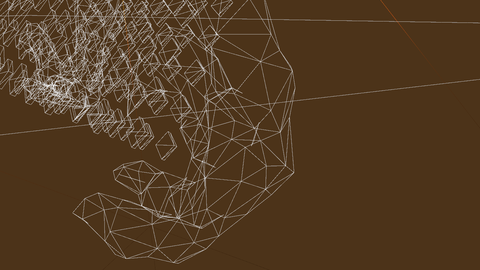
\includegraphics[width=0.5\textwidth]{resized/resized_Screenshot_raptorClaws_pure_WIRE.png} 
		wire frame	
		&
		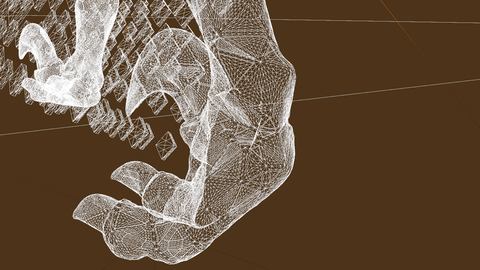
\includegraphics[width=0.5\textwidth]{resized/resized_Screenshot_raptorClaws_pure_WIRE_tess.png} 
		wire frame, tessellated
		\tabularnewline

		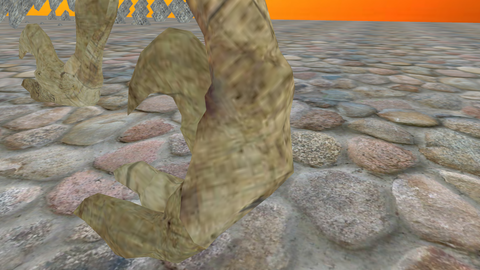
\includegraphics[width=0.5\textwidth]{resized/resized_Screenshot_raptorClaws_diffuseTex.png} 
		diffuse textured
		&
		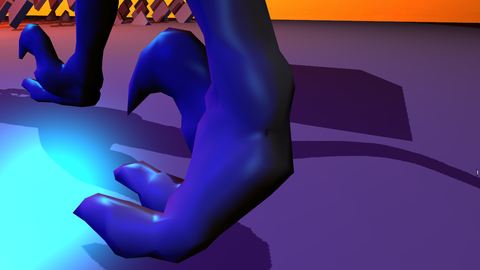
\includegraphics[width=0.5\textwidth]{resized/resized_Screenshot_raptorClaws_lighting.png}
		lighted
		\tabularnewline
		
		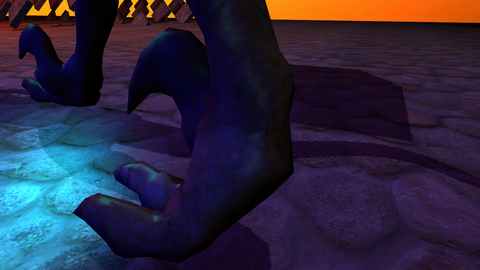
\includegraphics[width=0.5\textwidth]{resized/resized_Screenshot_raptorClaws_lighting_diffuseTex.png} 	
		lighted, diffuse textured
		&
		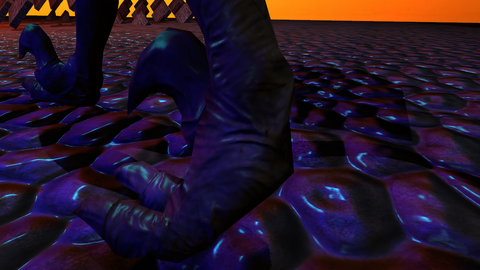
\includegraphics[width=0.5\textwidth]{resized/resized_Screenshot_raptorClaws_lighting_diffuseTex_normalMap.png}	
		lighted, diffuse textured, normal mapped
		\tabularnewline

		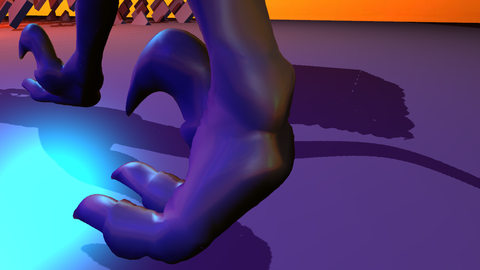
\includegraphics[width=0.5\textwidth]{resized/resized_Screenshot_raptorClaws_lighting_envmap_tess.png} 	
		lighted, environment mapped, tessellated
		&
		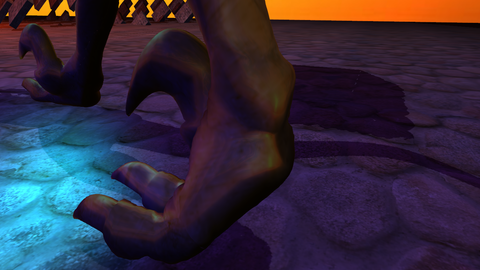
\includegraphics[width=0.5\textwidth]{resized/resized_Screenshot_raptorClaws_lighting_diffuseTex_envmap_tess.png}
		lighted, diffuse textured, environment mapped, tessellated
		\tabularnewline		
		
		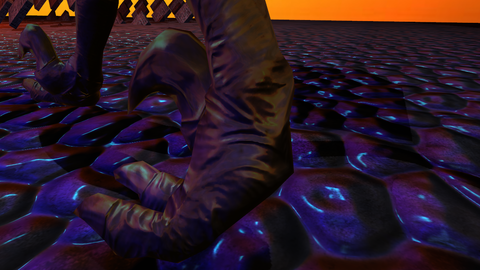
\includegraphics[width=0.5\textwidth]
			{resized/resized_Screenshot_raptorClaws_lighting_diffuseTex_normalMap_envMap.png} 	
		lighted, diffuse textured, normal mapped, environment mapped
		&
		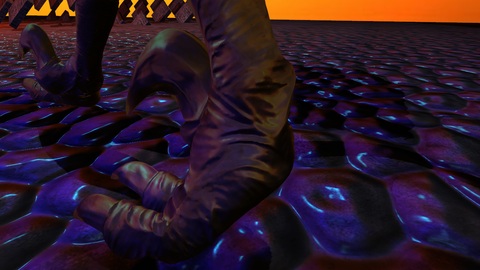
\includegraphics[width=0.5\textwidth]
			{resized/resized_Screenshot_raptorClaws_lighting_diffuseTex_normalMap_envMap_tess.png}		
		lighted, diffuse textured, normal mapped, environment mapped, tessellated
		\tabularnewline
	\end{tabular}
	\caption{Füße des Raptor-Modells, mit verschiedenen Permutationen aktivierter Shader-Features}
	\label{fig:shaderfeaturePermutations}
\end{figure}




\begin{figure}[!h]	 	
	\begin{tabular}{ x{0.5\textwidth} x{0.5\textwidth} }

   		\multicolumn{2}{ x{\textwidth} }{   			
    			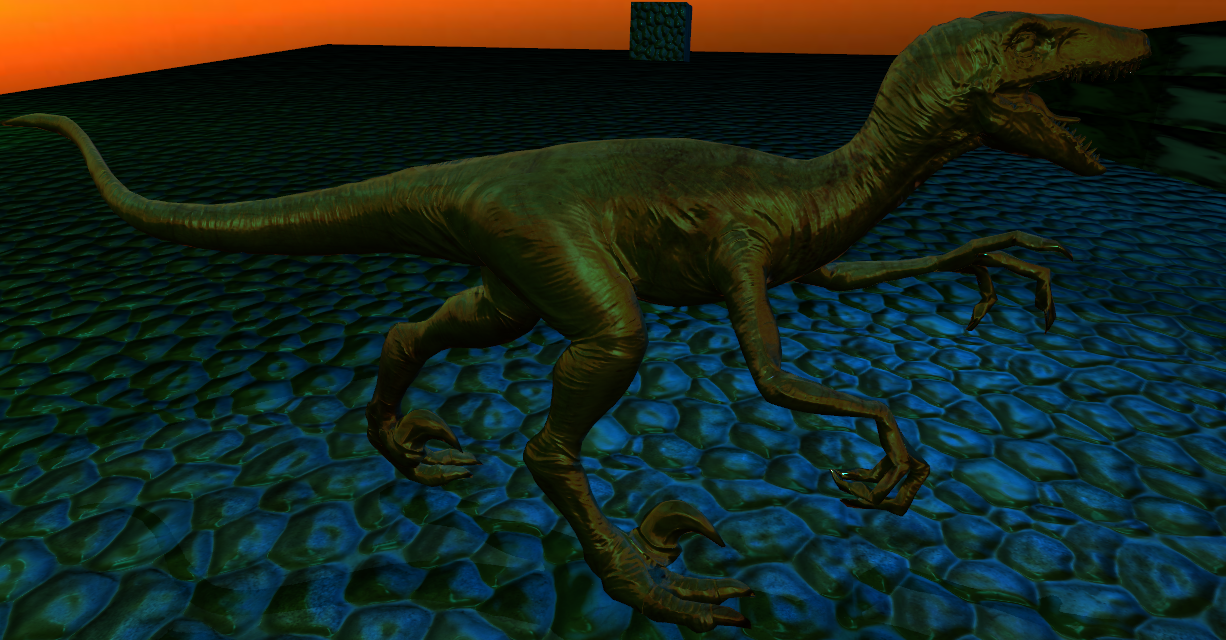
\includegraphics[width=\textwidth]{Screenshot_raptor_full.png} 
   		}	
   		\tabularnewline	
   		
   		\multicolumn{2}{ x{\textwidth} }{
    			Auf die Entfernung kann das Normal Mapping noch ausreichen,
		}
		\tabularnewline   		
		\multicolumn{2}{ x{\textwidth} }{
    			um Geometrie-Detail zu suggerieren ...
		}
		\tabularnewline
		
		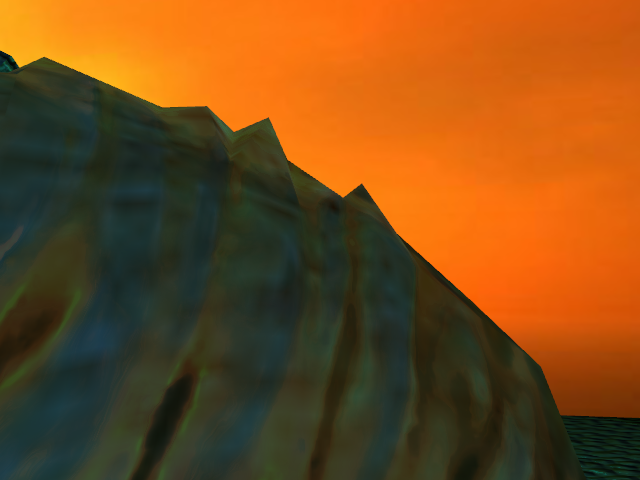
\includegraphics[width=0.4\textwidth]{Screenshot_raptorNeck_normal.png} 
		&
		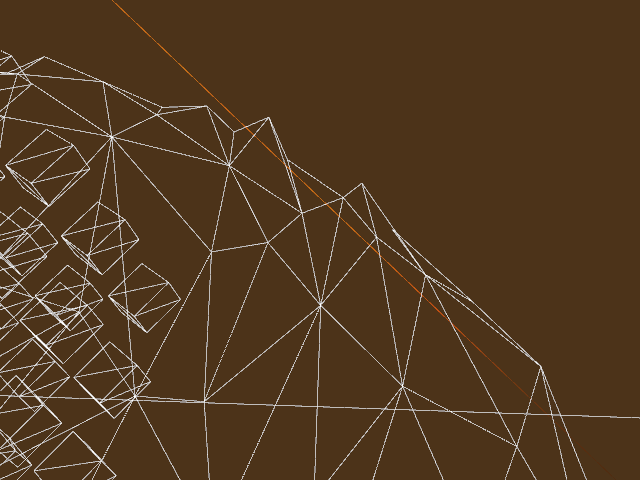
\includegraphics[width=0.4\textwidth]{Screenshot_raptorNeck_WIRE.png} 
		\tabularnewline
		
		\multicolumn{2}{ x{\textwidth} }{
			\multirow{1}{*}{
			... hier jedoch nicht mehr
			}
		}
		\tabularnewline
		
		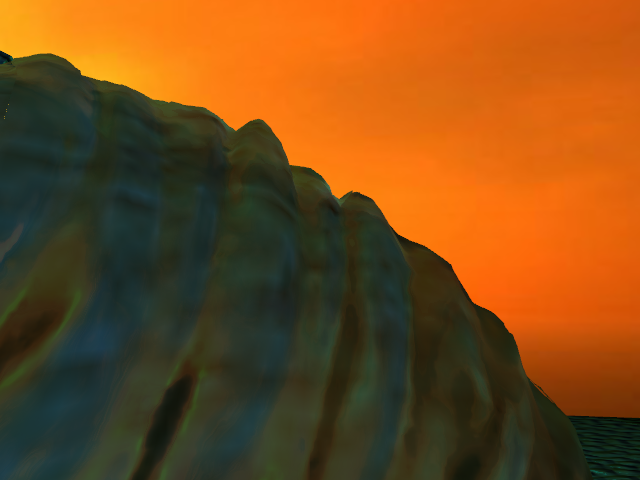
\includegraphics[width=0.4\textwidth]{Screenshot_raptorNeck_normaltess.png}
		&
		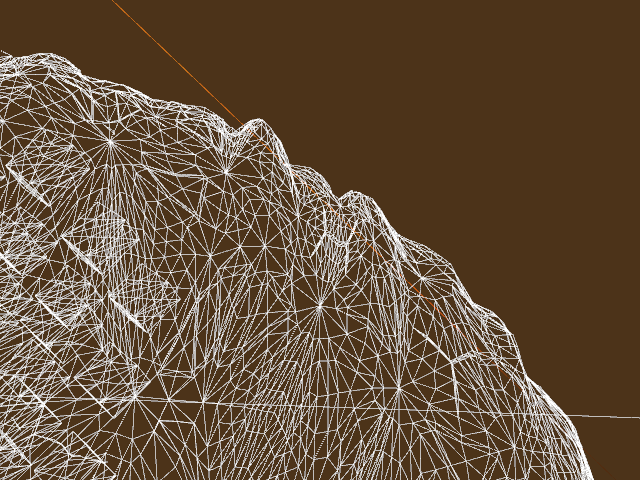
\includegraphics[width=0.4\textwidth]{Screenshot_raptorNeck_WIRE_tess.png}
		\tabularnewline

	\end{tabular}
	\caption{Gegenüberstellung des Detail-Grades mit und ohne Tessellation, Teil 1}
	\label{fig:gegenueberstellungTessNonTessCloseUpRaptorNeck}
\end{figure}


\begin{figure}[!h]	 	
	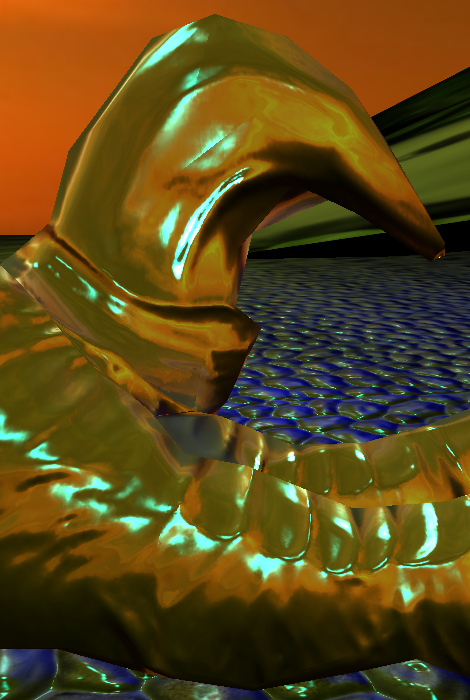
\includegraphics[width=0.5\textwidth]{Screenshot_raptorFootCloseUp_nonTess.png} 
	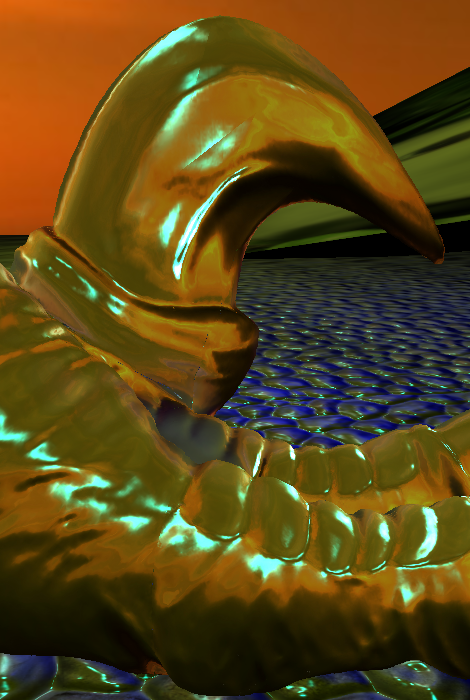
\includegraphics[width=0.5\textwidth]{Screenshot_raptorFootCloseUp_tess.png} 
	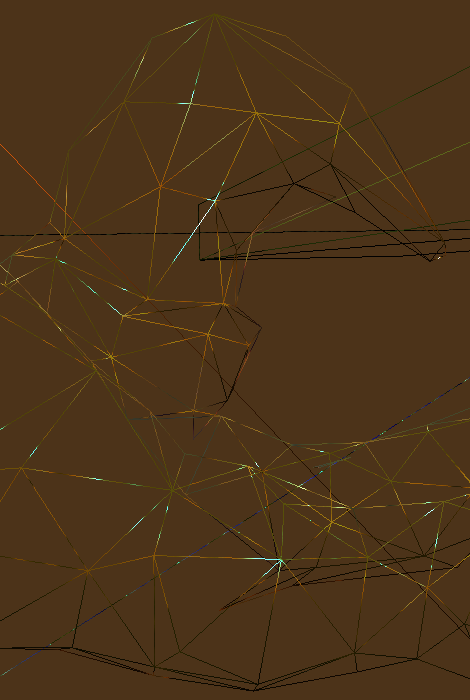
\includegraphics[width=0.5\textwidth]{Screenshot_raptorFootCloseUp_WIRE_nonTess.png} 
	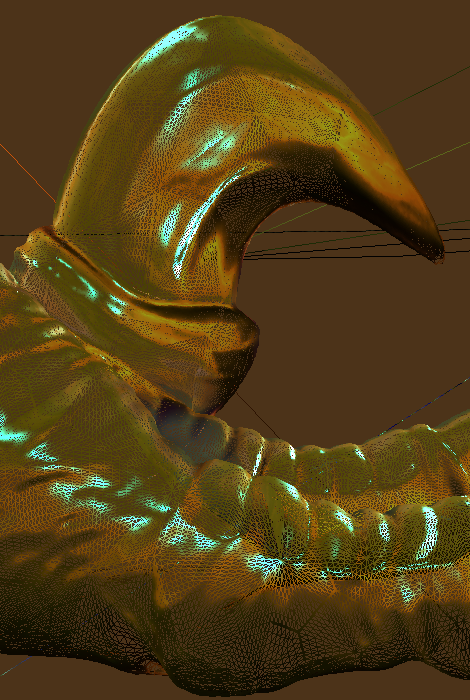
\includegraphics[width=0.5\textwidth]{Screenshot_raptorFootCloseUp_WIRE_tess.png} 

	\caption{Gegenüberstellung des Detail-Grades mit und ohne Tessellation, Teil 2}
	\label{fig:gegenueberstellungTessNonTessCloseUpRaptorFoot}
\end{figure}


\begin{figure}[!h]

	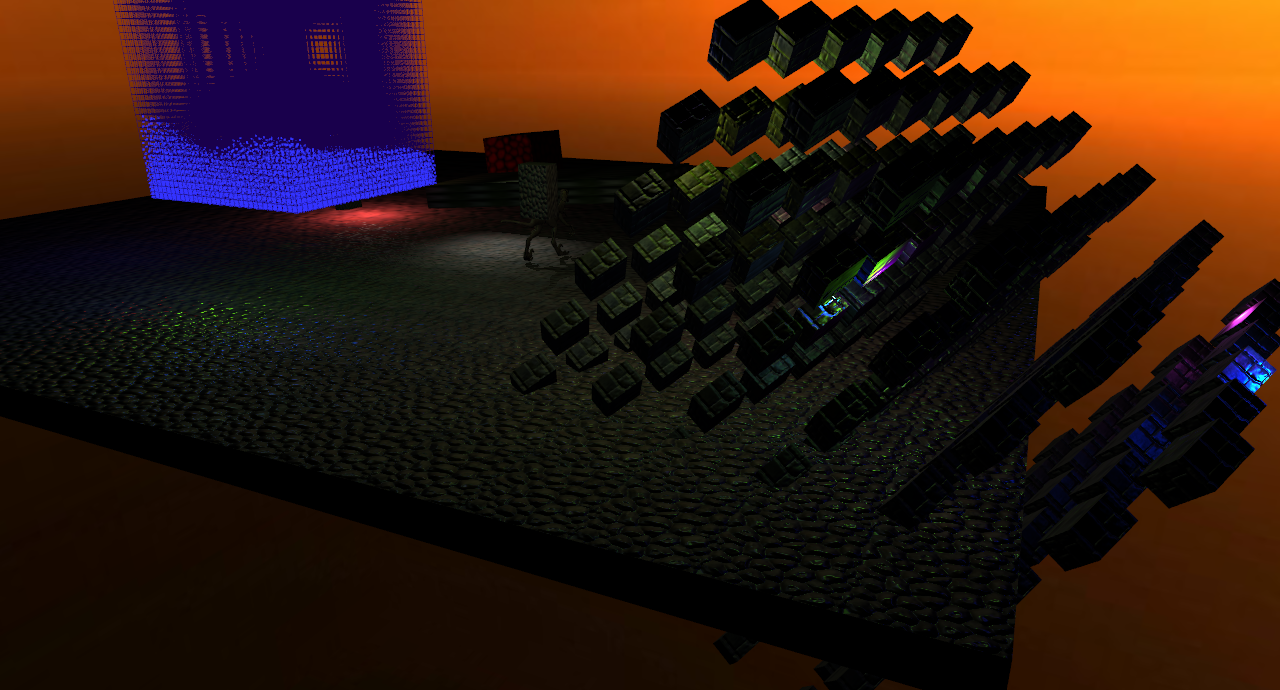
\includegraphics[width=1.2\textwidth]{Screenshot_Overview_40LS_LightingDiffuseTexNormal.png} 
	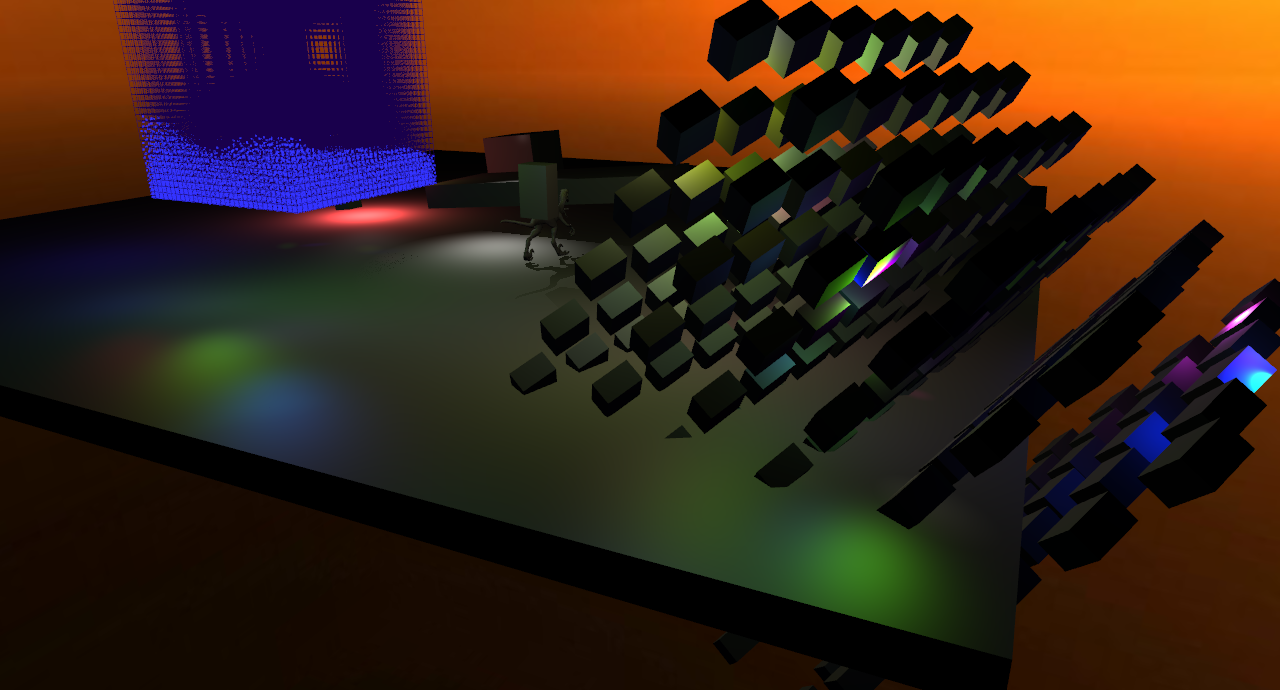
\includegraphics[width=1.2\textwidth]{Screenshot_Overview_40LS_Lighting.png}

	\caption{Überblick über die Scene, beleuchtet von 40 Lichtquellen; \\
	Mit Normal Mapping: 18 FPS; ohne Normal Mapping: 19 FPS\\
	(auch hier FPS ohne mechanische Simulation)
	}
	\label{fig:sceneOverview40LQ}
\end{figure}


\begin{figure}[!h]
	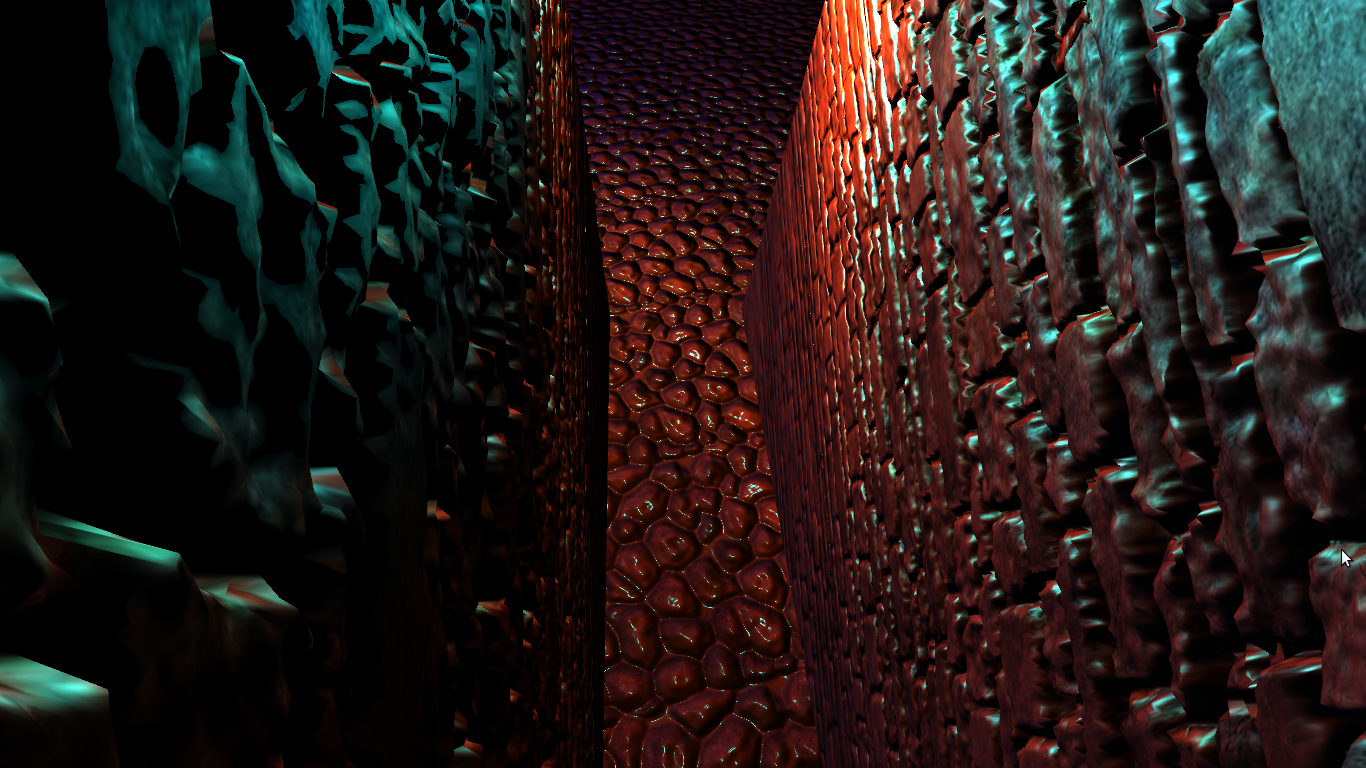
\includegraphics[width=1.0\textwidth]{Screenshot_LODwall_tess.png} 
	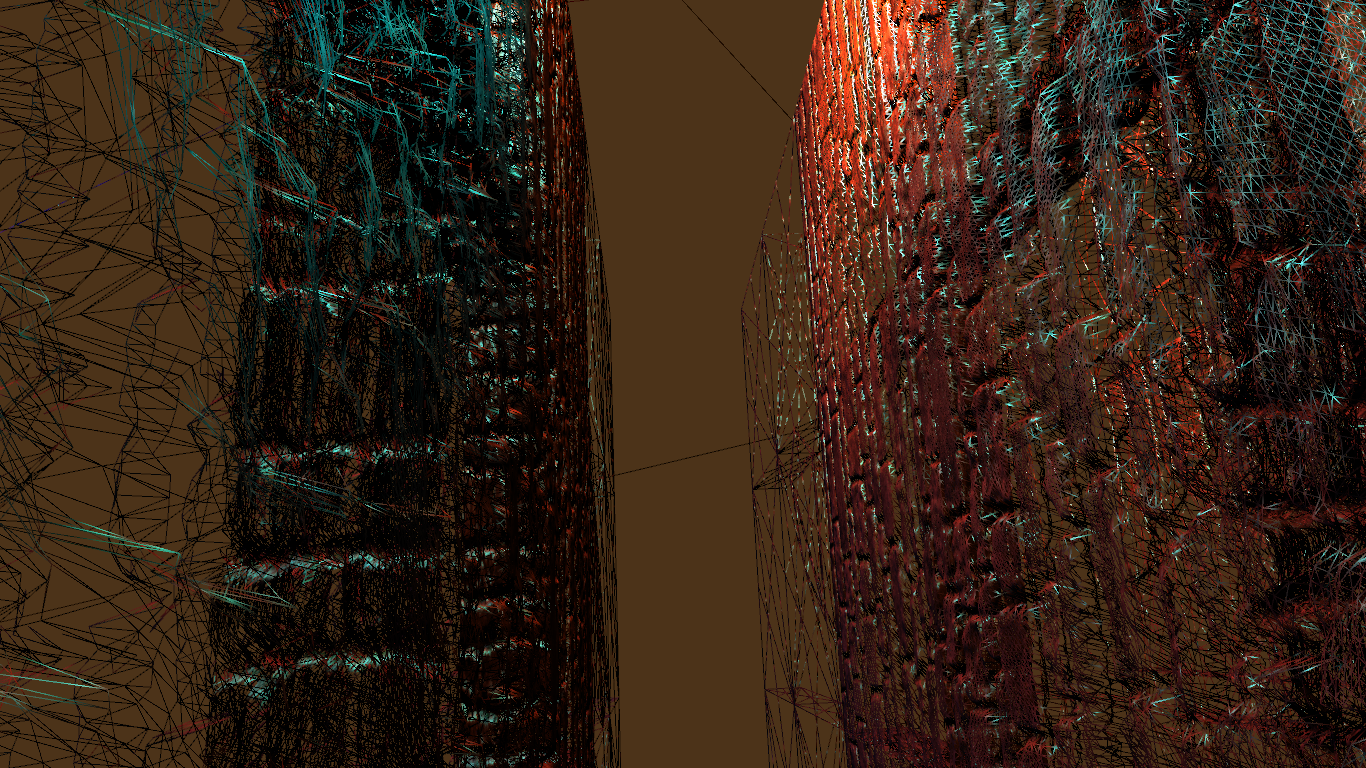
\includegraphics[width=1.0\textwidth]{Screenshot_LODwall_WIRE_tess.png}
	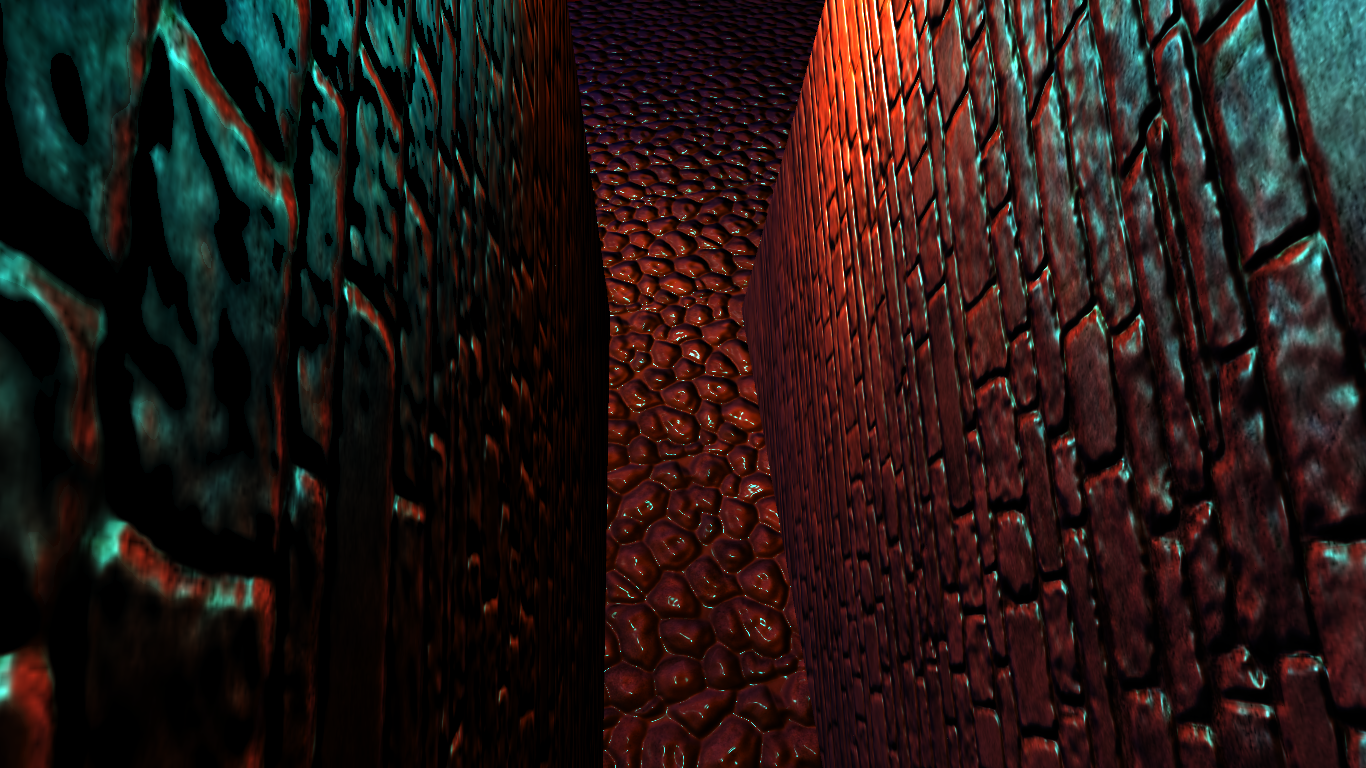
\includegraphics[width=1.0\textwidth]{Screenshot_LODwall_nonTess.png} 
	%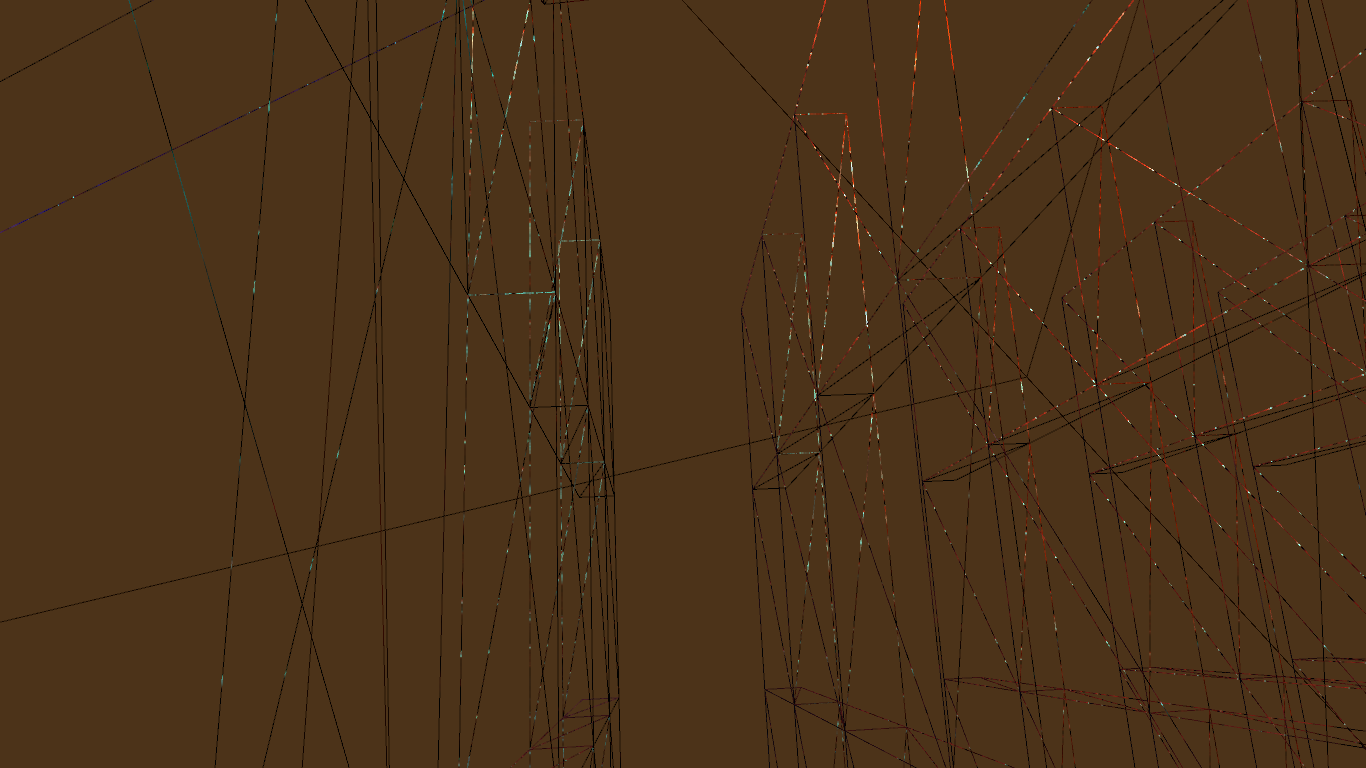
\includegraphics[width=1.0\textwidth]{Screenshot_LODwall_WIRE_nonTess.png}

	\caption{
		Oben: dynamisches Level of Detail dank Tessellation;\\
	 	Unten: Zum Vergleich ohne Tessellation
	}
	\label{fig:LODwall}
\end{figure}

\begin{figure}[!h]

	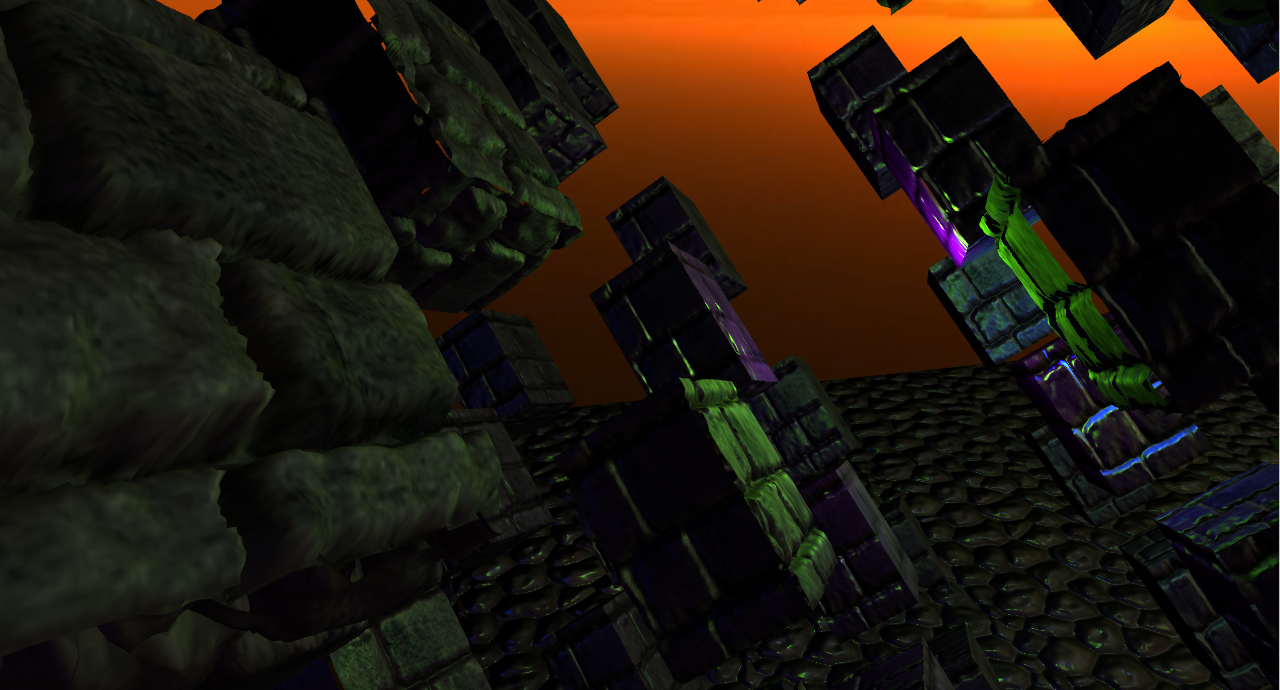
\includegraphics[width=1.0\textwidth]{Screenshot_instancedBoxesMiddle_40LS_tess.png} 
	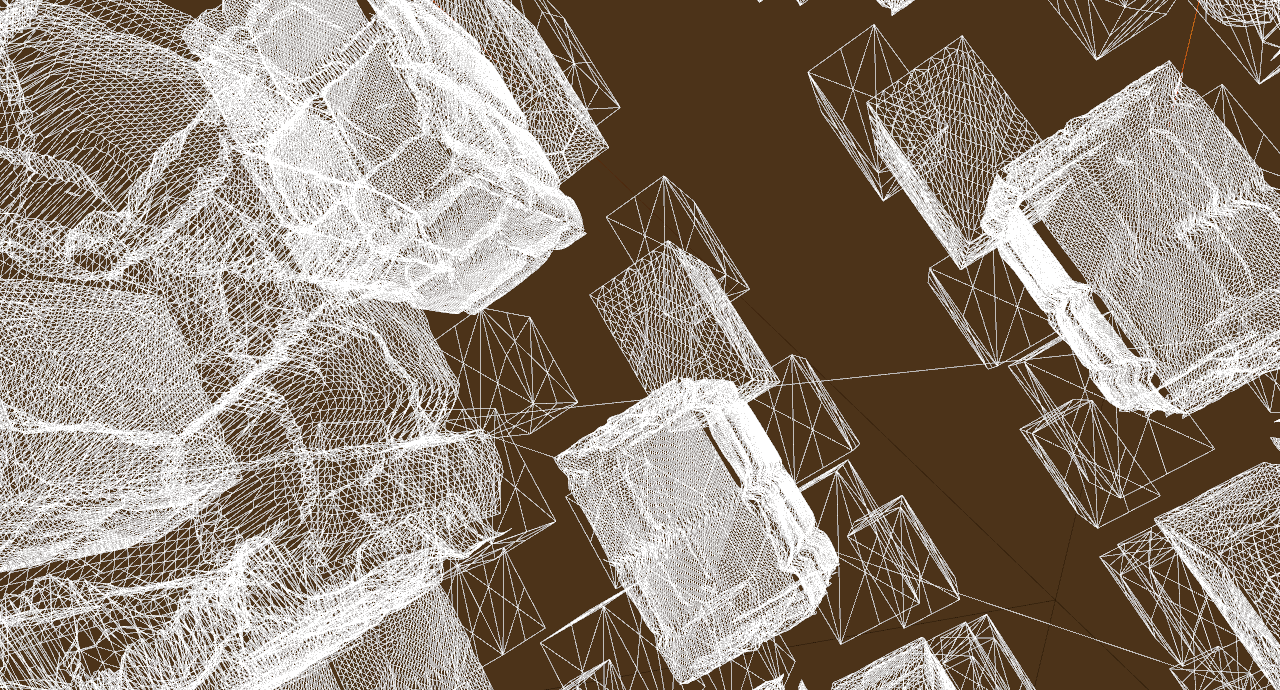
\includegraphics[width=1.0\textwidth]{Screenshot_instancedBoxesMiddle_40LS_WIRE_tess.png}
	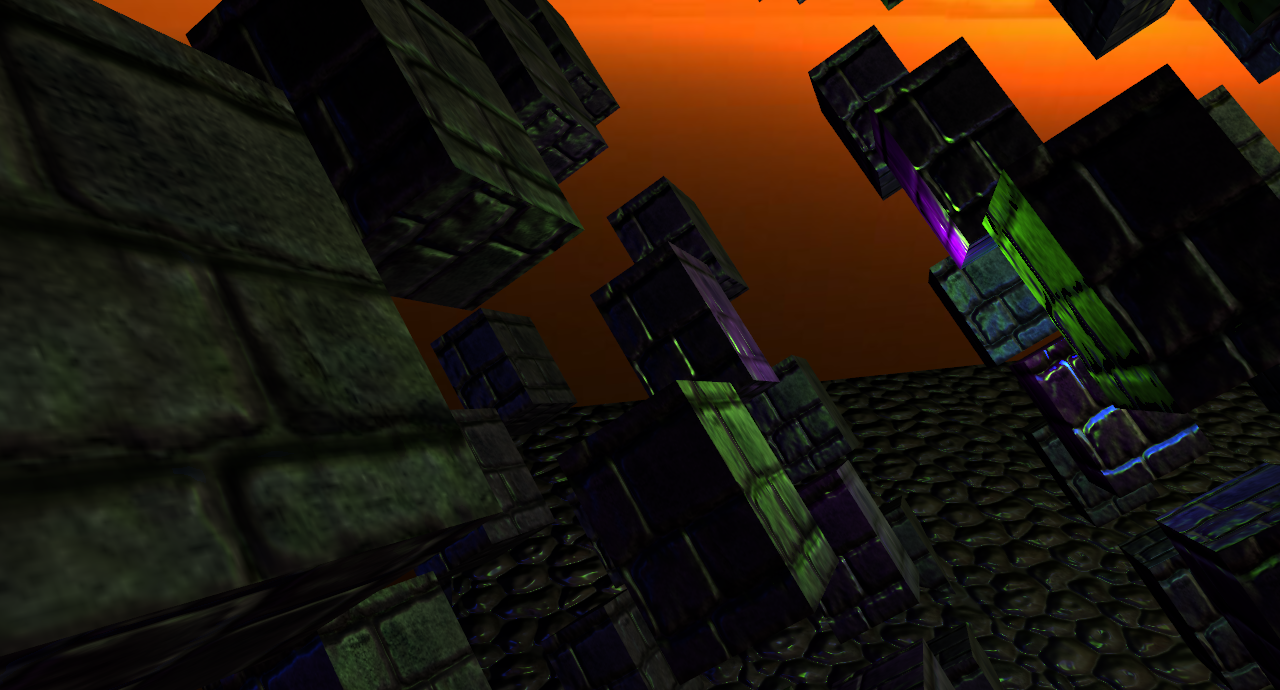
\includegraphics[width=1.0\textwidth]{Screenshot_instancedBoxesMiddle_40LS_nonTess.png} 
%	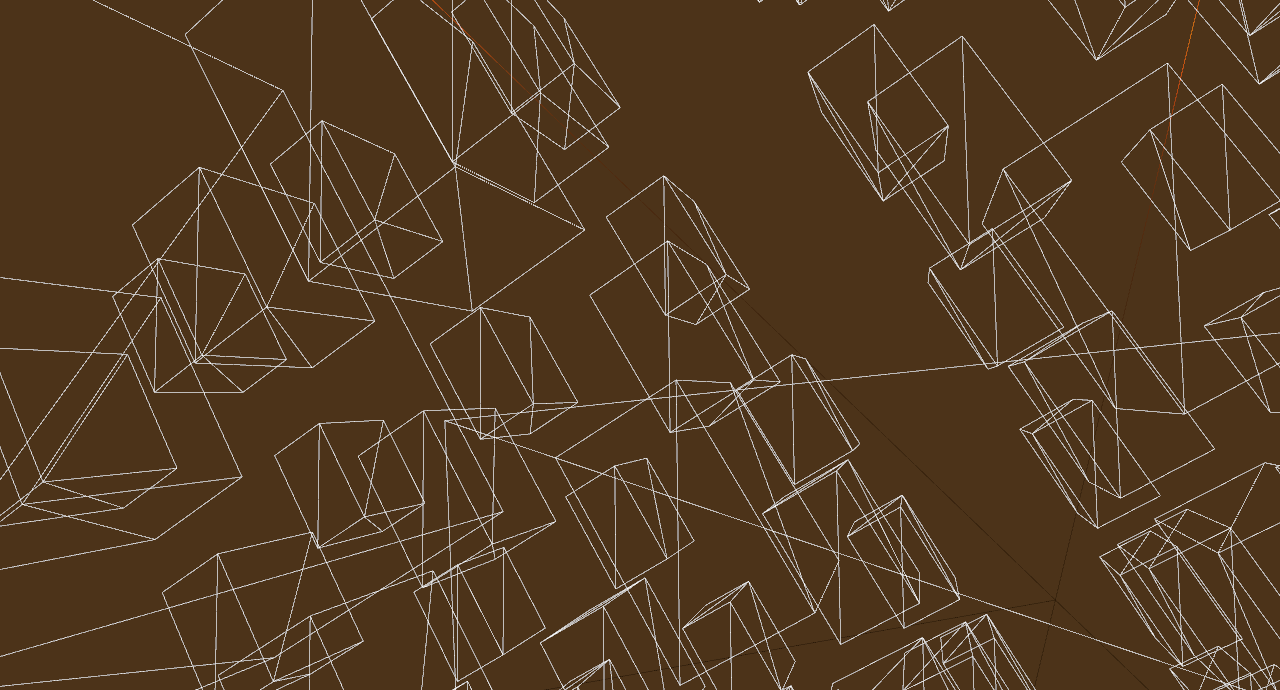
\includegraphics[width=1.0\textwidth]{Screenshot_instancedBoxesMiddle_40LS_WIRE_nonTess.png}

	\caption{ 
		Oben: dynamisches Level of Detail dank Tessellation, 40 Lichtquellen: 9 FPS; \\
	 	Unten: Zum Vergleich ohne Tessellation, 40 Lichtquellen: 20 FPS; 
	}
	\label{fig:instancedBoxesMiddle}
\end{figure}

%--------------------------------------------------------------------------------------------------------------------

\subsection{Fluid-Simulation}

	Bei der Fluid-Simulation mit OpenCL wird jetzt die verschiedene Hardware interessant:
	Tabelle \ref{tab:fluidSimPerformance} zeigt die durchschnittlichen Frames pro Sekunde
	mit verschiedenen Particle Counts auf den getesteten Devices, nachdem das Fluid einen repäsentativen
	Status erreicht hat, also seine Ruhe-Dichte, die vornehmlich vom SPH-Support-Radius und der Gas-Konstante abhängt
	\footnote{"`repräsentativ"' deshalb, weil in der Anfangsphase, wo das Fluid z.B. aus einer Säule zerfällt, die Partikel
	zeitweilig so komprimiert werden können, dass die Frame-Rate drastisch einbricht, weil bei vollen Grid-Zellen
	es dann sehr viele Nachbar-Partikel gibt, die alle heruntergeladen und verrechnet werden müssen.
	Beim Aufwand $O(N*M)$ steigt in diesem Falle das $M$ an. Ein weiteres Problem ist die Erzeugung vieler Work-Groups
	für die SPH-Kernels in diesem Fall, wo manche vielleicht nur wenige Partikel enthalten, 
	dennoch müssen der volle Kontrollfluss und die volle Bandbreite für die Beschaffung der Nachbar-Partikel 
	für eine Work Group genutzt werden. Die Verwaltung der Work Items in Warps à 32 Work Items, 
	die implizit synchronisiert sind, verschlimmert die Situation, da egal ob ein oder 32 Partikel 
	bearbeitet werden, die Anzahl an Berechnungen auf der GPU die gleiche ist.}.
	Die Fluid-Simulation ist so rechenaufwändig, dass das visuelle Rendering für die Benchmark-Ergebnisse fast keine 
	Rolle mehr spielt. Dennoch sei erwähnt, dass die Benchmarks in der im vorherigen Abschnitt gezeigten prototypischen
	Szene durchgeführt wurden, und zwar mit einer Auflösung von 1280*720, 4x Multisampling, 5 Lichtquellen zur Beleuchtung,
	eine davon mit Shadow Mapping-Funktionalität.
	
	\begin{table}[!h]
		\begin{tabular}{|l|c|r|r|r|}
		\noalign{\hrule}
		
		num. particles \textbackslash Device & cache-using impl. 	& GT 435M & GTX 280 & GTX 570  \\
		\noalign{\hrule}
		
		\multicolumn{1}{|c|}{
    		\multirow{2}{*}{$2^{15}$ ( 32768)}
    	}	 	 				& \checkmark 			&  6.0	  & 13.1	& 50.0	 \\
 								\cline{2-5}
 		\multicolumn{1}{|c|}{} 	& x						&  5.8	  & 13.0	& 45.0	 \\
 		\noalign{\hrule}   	
 		
 		\multicolumn{1}{|c|}{
    		\multirow{2}{*}{$2^{16}$ ( 65536)}
    	}	 	 				& \checkmark 			& 3.5	  & 7.7		& xxx	 \\
 								\cline{2-5}
 		\multicolumn{1}{|c|}{} 	& x						& 3.3	  & 7.2		& 27.0	 \\
 		\noalign{\hrule}   	
 		
 		\multicolumn{1}{|c|}{
    		\multirow{2}{*}{$2^{17}$ (131072)}
    	}	 	 				& \checkmark 			& 1.5	  & 3.6		& xxx	 \\
 								\cline{2-5}
 		\multicolumn{1}{|c|}{} 	& x						& 1.4	  & 3.4		& 14.0	 \\
 		\noalign{\hrule}   	
 		
 		\multicolumn{1}{|c|}{
    		\multirow{2}{*}{$2^{18}$ (262144)}
    	}	 	 				& \checkmark 			& 0.8	  & 1.7		& xxx	 \\
 								\cline{2-5}
 		\multicolumn{1}{|c|}{} 	& x						& 0.7	  & 1.8		& 6.0	 \\
 		\noalign{\hrule}   	
    	

		\end{tabular}
		\caption{		
			Performance der Fluidsimulation auf verschiedenen GPUs, mit implizit Cache-benutzender Implementation (direkte 
			Reads vom Global Memory) 
			und mit Local-Memory-nutzender Implementation wie in \cite{Goswami2010})
		}
		\label{tab:fluidSimPerformance}
	\end{table}
	\todo{überprüfen: GTX 280 @ 32k direct reading impl: inkonsitent}
	\todo{lub lass die cache-benchmarks ruberwachsen! :D}
	
	Zu Tabelle \ref{tab:fluidSimPerformance} ergeben sich etliche Beobachtungen:
	\begin{enumerate}
		\item Die Performance zwischen den beiden Fermi-Devices unterscheidet sich immer mindestens um den Faktor 7,
		was mit der Anzahl an Compute Units korrelliert (2 zu 14); Der über das Siebenfache hinausgehende
		Performance-Unterschied ist wohl der höheren Taktung und weiteren Desktop-GPU- vorbehaltenen Features zu verdanken.
		\item Aus der oberen Feststellung, dass die Performance mit der Anzahl an Compute Units zu korrellieren scheint,
		und nicht mit der Gesamt-Anzahl an Rechen-Einheiten (96 zu 480), mag zwei Gründe haben: Entweder sind die
		Kernels so voller Daten-Abhängigkeiten und Synchronisations-Punkte, dass die Superskalarität, die nötig ist, um 
		alle 48 Recheneinheiten einer solchen Compute-Unit zu nutzen 
		\footnote{Work Items sind auch bei diesen Chips in "`Warps"' à 32 Work Items organisiert und synchronisiert, so 
		dass weitere Recheneinheiten nur durch Ausnutzen von Superskalarität 
		(also paralleler Ausführung von eigentlich sequentiellen Befehlen, zwischen denen aber keine Abhängigkeiten
		bestehen) genutzt werden können.}
		, nicht mehr gegeben ist;
		oder aber der Unterschied ist noch stärker der höheren Taktung und weiteren Stärken der GTX 570 zu verdanken.
		\item Der Perfomance-Unterschied zwischen der GT435M und der GTX 280 liegt nur bei einem Faktor von gut 2,
		obwohl die GTX280 mehr als doppelt so viele Recheneinheiten (96 zu 240) hat und zum Release der GT200-Generation
		das Flaggschiff darstellte, wohingegen die GT435M innerhalb der Fermi-Generation nur eine Midrange-Notebook-GPU
		repräsentiert. Nvidia hatte für die Fermi-Generation u.a. mit sehr guter Performance bei Fluid-Simulationen
		geworben. Gründe für die relativ deutlich bessere Performance pro Recheneinheit zwischen GT200 und Fermi-
		Architektur 
		\footnote{
			zwischen GTX280 und GTX 570 :  
			$(240/480)$ Recheneinheiten $ \times 3 $ mal bessere Performance $ \approxeq 1.5 $ \\
			bzw. wischen GTX280 und GT 435M :  
			$(240/96)$ Recheneinheiten $ \times 0.5 $ mal bessere Performance $ \approxeq 1.25 $
		} können u.a. sein:
		\begin{enumerate}
			\item Der L1-Cache der Fermi-Architektur, der bei Global Memory Reads Latenz verkürzt und Bandbreite spart
			\item Die verbesserte Integer-Performance: Durch die Verwaltung der Beschleunigungs-Struktur über Z-Indices,
			Radix Sort, Stream Compaction etc. bestehen viele Kernels ausschließlich aus Integer-Operationen.
			Nativ sind bei GT200 nur 24Bit-Integer-Multiplikationen unterstützt, die ich nicht explizit genutzt habe, weil 
			ich für Fermi optimieren wollte; hier würde sich die Performance durch diese Operationen sogar 
			verschlechtern (\cite{nvidiaOpenCLProgrammingGuide}, S. 34). Ein Makro könnte das 
			Architektur-spezifische Problem beheben, noch wird aber keines verwendet.
			\item Der größere Local Memory der Fermi-GPUs:
				Hierdurch kann eine Work Group z.B. mehr Radix Counters beim Radix Sort pro Work Group haben, 
				was die lokalen Scan-Intervalle größer und effektiver macht, denn ein großer Scan pro WorkGroup 
				hat in den letzten Scan-Schritten nur noch eine aktive Warp, wohingegen bei vielen kleinen Scans pro Work 					Group am Ende so viele Warps aktiv sind, wie lokale Radix-Counter-Intervalle gleichzeitig pro Work Group 	
				gescannt werden; Außerdem nimmt mit größeren "`Local Scan"'-Intervallen die Anzahl der Elemente für den
				"`Global Scan"' ab, so dass auch dieser schneller geht.
			\end{enumerate}	
	\end{enumerate}
	
	
	
	
	
	
	Ich habe mich bei meiner OpenCL-Implementation, wie erwähnt, soweit es mir technisch möglich war (erinnere: Buffer als
	Textur binden geht in OpenCL nicht) und sinnvoll erschien
	\footnote{manche Papers waren noch auf die G80- Architektur
		ausgelegt, die Vorgänger-Generation vom GT200, welche noch sehr anfällig für nicht absolut 
		"`aligned memory access Patterns"' war und außerdem keine atomaren Operationen unterstützte},
	sowohl algorithmisch an Goswami (\cite{Goswami2010}) orientiert, als auch wie er den 
	"`Work Efficient Parallel Scan"' aus \cite{Harris2007} implementiert, der die Basis für den in \cite{Grand2008} 
	erläuterten Parallel Radix Sort bildet, den wir ebenfalls beide nutzen.
	Die Implementationen sind also durchaus vergleichbar.
	
	\cite{Goswami2010} erreicht jedoch auch bei 256000 Partikeln ohne Visualisierung noch 10 FPS auf einer GTX280,
	wohingegen meine aktuelle OpenCL-Implementation auf dieser GPU nur 1.8 FPS erreicht, 
	also mehr als fünf mal langsamer ist.
	Dies hat vermutlich folgende Gründe:
	\begin{enumerate}
		\item Ich habe nicht explizit für GT200 optimiert, sondern meine Ziel-Architektur ist Fermi;
		somit habe ich wie gesagt nicht Operationen wie \lstinline|mul24(gentype x, gentype y)| verwendet,
		um die Integer-Performance zu erhöhen.
		\item Ich habe noch nicht die Optimierung eingebaut, welche die Dichte-Berechnungen im selben
		Kernel ausführt wie die Kraft-Berechnungen; Da mit einem SPH-Kernel ein signifikanter 
		Anteil an Kontrollfluss und	Bandbreite verbunden ist, erwarte ich hiervon eine Performance-Steigerung von 
		bis zu 1.5.
		\item Um den Bug, der auf Seite \pageref{enum:oclSyncBug} beschrieben ist, einzukreisen, wurde viel unnötiger 
		Synchronisations-Code ins Host-Programm eingestreut. Die Löschung diese sollte jedoch
		für die Performance kaum signifikant sein.\\
		Allerdings war in den Kernels zur Zeit der Benchmarks noch viel Code vom Typ
		\begin{lstlisting}
if(any(isnan(ownAccelerationNew)) || any(isinf(ownAccelerationNew)) ) 
	{ownAccelerationNew =  (float4)(0.0f,0.0f,0.0f,0.0f); }
		\end{lstlisting}
		, um etwaige "Not A Number"'s oder "`Infinities"' herauszufiltern; 
		
		\item
		Durch den auf Seite \pageref{enum:oclSyncBug} beschriebenen Bug laufen sowohl die "`Global Scan Phase"'
		des Radix Sort als auch der Scan, der die Stream Compaction vorbereitet, mit nur einer Work Group.
		Diese Kernels sind allerdings im Vergleich zu anderen nicht sonderlich aufwändig.
		
		
		\item Ich habe einen deutlich höheren Bandbreiten-und Speicher-Bedarf durch die Verwendung des 
		\emph{Velocity Verlet}- Integrations-Schemas, der das Durchschleifen von \emph{zwei} Geschwindigkeitswerten
		(predicted/corrected) und der Beschleunigung benötigt; Ferner verlangt meine konzipierte
		Unterstützung für mehrere Fluide zusätzlich folgende  Buffers:
		\begin{lstlisting}
//tracking buffer for fluid objects and rigid bodies to find their belonging particles in the
//recurrently reordered attribute buffers;
//used during (at least fluid) rendering as OpenGL index buffer;
//no ping pong necessary as no read/write or similar hazard can occur;
Buffer* mParticleIndexTableBuffer;
//used to associate a particle with its owning fluid or rigid body object
//and its particle ID within this object;
PingPongBuffer* mObjectInfoPiPoBuffer; //uint ping pong buffer	
		\end{lstlisting}
		Weil Scattered Writes auf der GPU aufgrund des fehlenden Coalescings extrem teuer sind,
		und Speicherbandbreite ohnehin im Vergleich zur reinen Rechenleistung schnell zum Flaschenhals
		zu werden droht, sind diese vier Buffers, von denen drei auch noch PingPong-Buffers und zwei
		sogar vier-Komponenten-Buffers sind, vermutlich enorm teuer durchzuschleifen. Wie im Ausblick
		aufgelistet, hat die Befreiung vom \emph{Velocity Verlet}-Verfahren eine der höchsten 
		Prioritäten \footnote{Für Gischt-Rendering nach \cite{Green2009FluidRenderingCurvatureFlow} ist die 
		Beschleunigung zwar relevant, muss aber dann nicht mehr zwischen den Simulations-Schritten gescattert
		werden; außerdem reicht vielleicht ein skalarer Wert zur Bestimmung des "`Gischt-Faktors"'}.
		Die beiden Buffers aus dem oberen Listing sind jedoch für die erweiterte Logik der Simulation erforderlich .
		\todo{ins paper schauen und uberprüfen falls zeit ist}
		
		\item 
		\label{enum:goswamiAccessPattern}
		Der vermutlich größte Flaschenhals meiner Implementation:
		Ich iteriere sequentiell über alle 27 Nachbar-Zellen und lade pro Iterations-Schritt parallel in Portionen
		à bis zu 32 Partikeln die Attribute der Nachbar-Partikel auf den Local Memory herunter.
		Dies mache ich, weil nach diesem Ansatz die Zugriffe auf den GPU-RAM coalesced sind.
		Goswami bindet jedoch in CUDA einen generischen Buffer an eine Texture-Unit,
		was den Vorteil hat, dass die Zugriffe über eine Texture Unit auch bei der GT200-Generation 
		gecachet sind und eine definierte Latenz 
		haben (und zwar die Latenz des Global Memories, was eigentlich schlecht ist, aber vielleicht wird das Scheduling 
		hierdurch effizienter). Durch diesen Umstand ist das Coalescing der Speicherzugriffe nicht mehr so wichtig,
		und er verwendet das folgende  Access Pattern: Er iteriert nicht über die 27 Nachbarzellen, sondern über die
		maximale Anzahl an Partikeln, die sich in einer der Nachbar-Zellen befindet, und lädt dann pro 
		Iterationsschritt parallel aus jeder Nachbarzelle ein Partikel herunter (sofern noch nicht jedes Partikel 
		in der entsprechenden Zelle abgearbeitet wurde). 
		Somit lädt er zu Beginn pro Iterations-Schritt fast immer 27 Partikel-Attribute parallel herunter, 
		aus jeder Nachbar-Zelle eines.
		Den Vorteil dieses Patterns habe ich während meiner Implementation verkannt: Wenn deutlich weniger
		als 27 Partikel in jeder Nachbar-Zelle sind, hat die Schleife deutlich weniger Iterationen. 
		Meine Implementation hat immer 27 Iterationen, selbst wenn alle Nachbarn-Zellen leer sind.
		Ich dachte, Verzicht auf Coalescing wäre schlimmer als ein komplexerer Kontrollfluss. 
		Außerdem dachte ich, dass die Performance am besten ist, wenn in jeder Zelle so viele Partikel sind,
		wie eine Warp groß ist, nämlich 32, denn bei geringerer Partikelzahl sind viele Recheneinheiten im Idle.
		Doch es hat sich herausgestellt, dass trotz des "`inhärenten Idles"' die Performance besser ist, wenn
		deutlich \emph{weniger} als 32 Partikel in einer Zelle sind. Dies entspricht der Faustregel,
		dass ein SPH-Partikel in etwa mit 33 Nachbar-Partikeln interagiert. Wären in jeder Zelle 32 Partikel,
		wären es 27*32=864 Nachbarn. Ich habe die Rolle der GPU als "`Number Cruncher"', den man vor allem
		vor nicht-gebündelten Speicherzugriffen bewahren und dessen Recheneinheiten man allesamt ausnutzen sollte,
		überschätzt.
		Wenn nur etwa 8 Partikel in einer Zelle sind, damit (außer zum Nachbar-Partikel-Herunterladen)
		ein Viertel der Recheneinheiten der GPU immer im Idle ist, ist die Performance besser als bei Voll-Auslastung
		durch überall knapp 32 Partikel (ich habe dieses Phänomen jedoch nicht systematisch auf ein Optimum hin 	
		untersucht).
		Die Warp-Größe von 32 scheint suboptimal für SPH zu sein. Dennoch ist die Parallelität der GPU
		immer noch hoch genug, um die CPU zu überflügeln.\\
		Letztendlich hätte das jetzige Benchmark-Ergebnis meiner OpenCL-SPH-Implementation
		auf einer GPU der GT200-Generation vermutlich auch nicht besser ausgesehen, wenn ich diese 
		jetzigen Erkenntnisse schon früher gehabt hätte. Denn es bleibt das Problem: man muss sich in
		OpenCL zwischen Buffer oder Textur entscheiden.
		 Das Pattern des zweimaligen Toggles der Particle-Attrbibute-Buffers
		(einmal nach Reordering, einmal nach Integration) könnte ermöglichen, dass man statt PingPong-Buffers
		einen generischen Buffer und eine Textur verwendet, weil in jedem Simulationsschritt jede Komponente
		des Ping Pong Buffers die gleiche Rolle hat. Dann kommt aber schon die nächste Beschränkung von
		OpenCL: Es gibt keine 1D-Texturen. Man muss also dann den linearen Speicher auf 2D-Textur-Koordinaten
		übertragen. Intellektuell ist dies möglich, wäre aber eine bittere Pille in Bezug auf konsitente Paradigmen.
		Vielleicht werden zukünftige OpenCL-Spezifikationen 1D-Texturen und Binden von Buffern an Texture-Units
		ermöglichen, jetzt jedoch bliebe auf GT200 nur dieser Trick, den ich aufgrund meines Fokus auf Fermi vorerst 
		nicht bereit bin, zu probieren.
		Da die Fermi-Architektur auch für den Non-Textur-Speicher einen Cache hat, hat sich ab dieser
		Hardware-Generation die 
		oben breit erläuterte Problematik womöglich erledigt. Ich werde das Access Pattern von Goswami
		ausprobiern, und dabei  rein lineare Buffer benutzen. Die Gefahr ist hier, dass der Cache zu klein ist
		(16 kB) und für Dinge wie Register Spilling genutzt werden könnte. Dies muss man wohl einfach ausprobieren,
		solange man keinen Einblick in Hardware und Treiber hat.
		Ob das Partikel -Access Pattern von Goswami allerdings auch auf Fermi-Devices irgendwelche Vorteile bringt, 
		vermag ich noch schwer abzuschätzen. Auf eine weitere Erörtung sei hier verzichtet.
		
	\end{enumerate}	
	
%-------------------------------------------------------------------------------------------------------------

	Was sehr überrascht, ist der Umstand, dass selbst auf der GTX 280 die OpenCL-Implementation schneller läuft, die 
	\emph{nicht} die Attribute der Nachbar-Partikel coalesced in den Local Memory herunter lädt, um dann 
	mit Register-Latenz für die SPH-Berechnungen zur Verfügung zu stehen; auch diese GPU
	bringt mehr Leistung, wenn jedes Nachbar-Attribut direkt vom Global Memory gelesen wird.
	Dieses Phänomen kann ich mir nur durch folgende Hypothesen erklären:
	\begin{enumerate}
		\item Mein Access Pattern (s.o., S. \pageref{enum:goswamiAccessPattern}) ist vielleicht so suboptimal
		(Kontrollfluss- und Snychronisations-aufwändig), dass
		der Synchronisationsaufwand den Vorteil der coalesced Reads aufwiegt. 
		Sobald ich das Access Pattern in meiner Implementation angepasst habe, wird diese Hypothese
		entweder bestätigt oder verworfen.
		\item Der OpenCL-Compiler ist womöglich so ausgefeilt, dass er in der Schleifen-Laufvariable, die in die Index-
		Berechnungen der Global Memory Reads einfließen, ein sequentielles Pattern erkennt und automatisch
		die Speicher-Zugriffe so optimiert, dass ein oder mehrere "`Strides"' eines globalen Speicher-Transfers
		(je nach Compute-Capability ist ein Stride 32-128 Byte groß, egal ob man nur ein Byte oder alle benötigt) 
		automatisch lokal zwischengespeichert werden, ohne dass der aufwändige Kontrollfluss- und Synchronisations-Code 
		ausgeführt werden muss.
		\item Der Aufwand durch Kontrollfluss, Synchronisation und SPH-Berechnungen ist 
		(nicht zuletzt durch das momentane Access Pattern) so
		groß, dass der L2-Cache aureicht, um die Latenz zu verstecken, und ein Download in den Local Memory
		in diesem Sinne	gar keinen Vorteil bringt, sondern viel mehr der Snychronisations- und Kontrollfluss-Code
		die Geschwindigkeit weiter ausbremst.
	\end{enumerate}
	Es sei betont, dass dies reine Spekulationen sind.\\
	
	


%---------------------------------------------------------------------------------------------------	
	
	
	Zusammenfassend kann man sagen, dass die Performance meiner SPH-Implementation nicht gerade hoch erfreulich ist, 
	es jedoch noch genügend Stellschrauben gibt, um etwas dagegen zu tun.\\
	
	
	\todo{diesen inhalts-kram in simulations-section auslagern, sobald skelett steht; habs erstmal hierhin gedumpt, fdalls 
	ich das kapitel gar nicht mehr schaffe}


\begin{figure}[!h]
	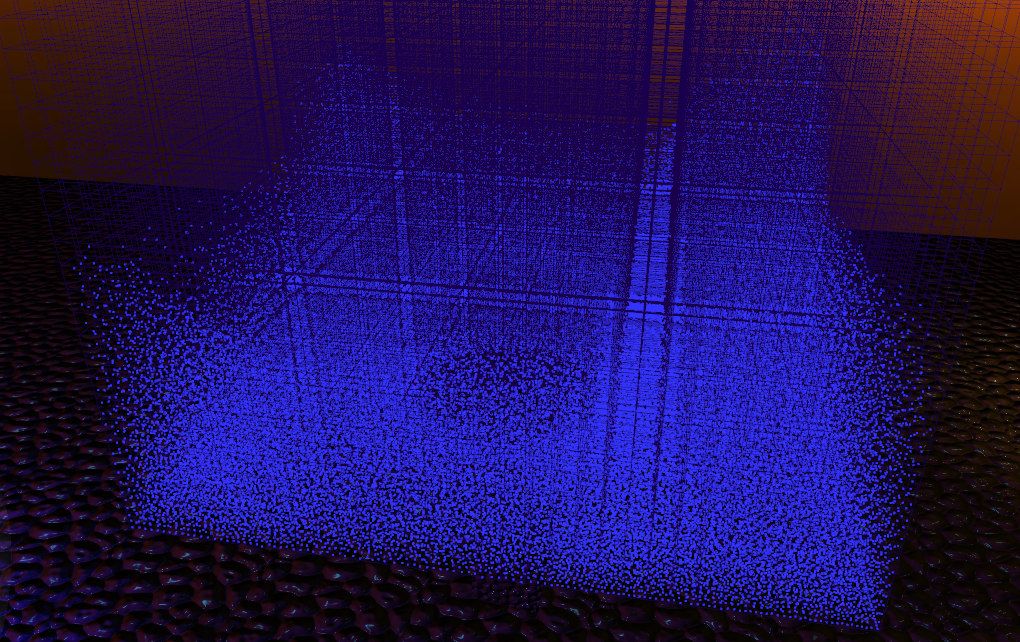
\includegraphics[width=1.0\textwidth]{fluidKraftFeldInit.png} 
	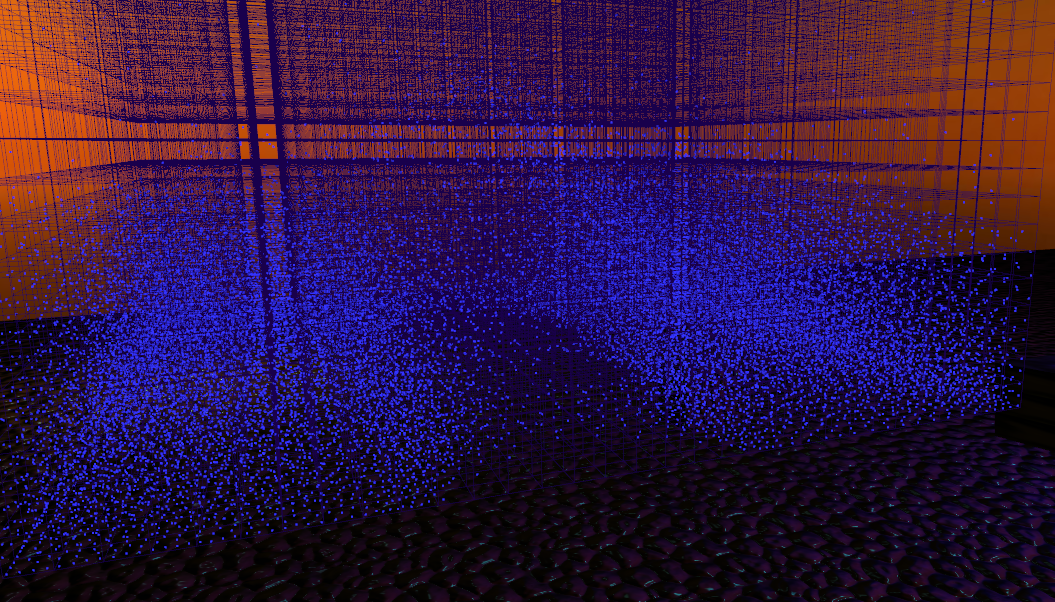
\includegraphics[width=1.0\textwidth]{fluid_Schneise.png}
	\caption{ 
		Fluid-Benutzer-Interaktion:\\
		Oben: Benutzer hat gerade per Mausklick ein kugelförmiges Kraftfeld erzeugt;\\
		Unten: Benutzer hat ein Kraftfeld vor sich durch Gedrückt-Halten der Maustaste aufrecht erhalten
		und damit nach Navigation durch das Fluid eine Schneise geschlagen
	}
	\label{fig:fluidSimForcePix}
\end{figure}

\begin{figure}[!h]
	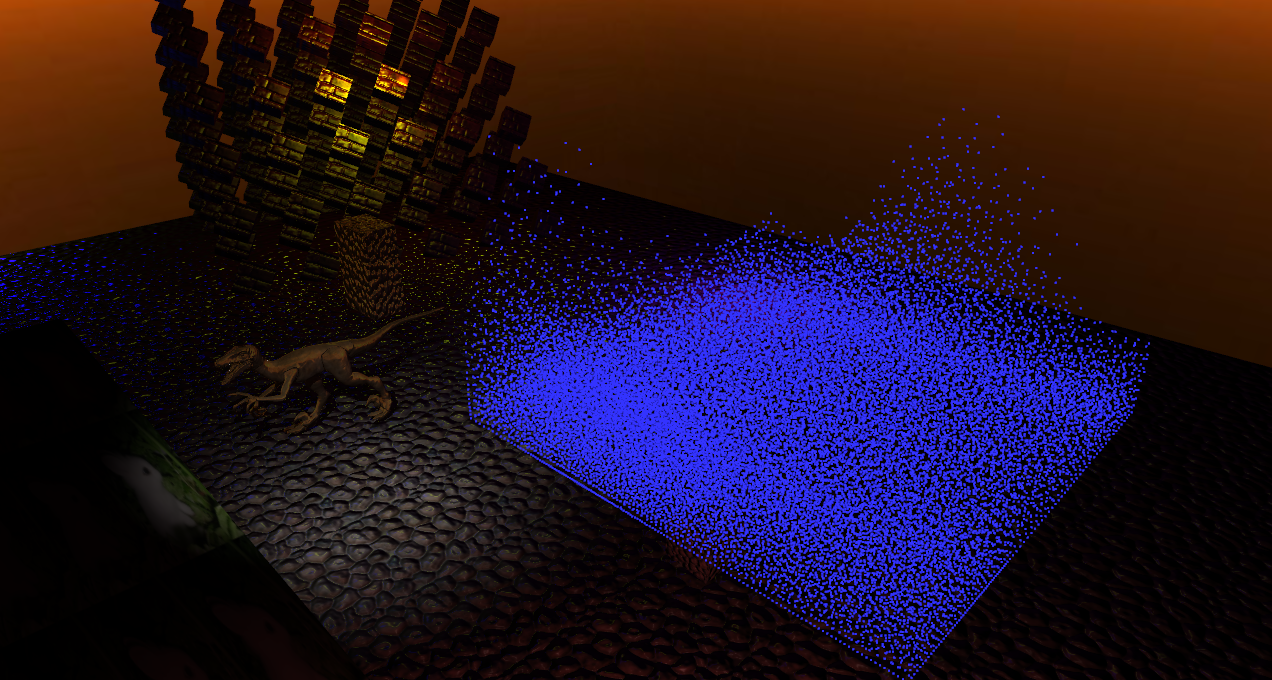
\includegraphics[width=1.25\textwidth]{fluidNoGrid.png} 
	\caption{ 
		Fluid ohne Darstellung des Uniform Grid
	}
	\label{fig:fluidNoGrid}
\end{figure}







\clearpage
